%%% Template originaly created by Karol Kozioł (mail@karol-koziol.net) and modified for ShareLaTeX use

\documentclass[a4paper,11pt]{article}

\usepackage[T1]{fontenc}
\usepackage[utf8]{inputenc}
\usepackage{graphicx}
\usepackage{xcolor}

\renewcommand\familydefault{\sfdefault}
\usepackage{tgheros}
% \usepackage[defaultmono]{droidmono}

\usepackage{amsmath,amssymb,amsthm,textcomp}
\usepackage{enumerate}
\usepackage{multicol}
\usepackage{tikz}

\usepackage{geometry}
\geometry{left=15mm,right=15mm,%
bindingoffset=5mm, top=15mm, bottom=25mm}


\linespread{1.3}

\newcommand{\linia}{\rule{\linewidth}{0.5pt}}

% custom theorems if needed
\newtheoremstyle{mytheor}
    {1ex}{1ex}{\normalfont}{0pt}{\scshape}{.}{1ex}
    {{\thmname{#1 }}{\thmnumber{#2}}{\thmnote{ (#3)}}}

\theoremstyle{mytheor}
\newtheorem{defi}{Definition}

% my own titles
\makeatletter
\renewcommand{\maketitle}{
\begin{center}
\vspace{2ex}
{\huge \textsc{\@title}}
\vspace{1ex}
\\
\begin{center}
    \@author
\end{center}
\end{center}
}
\makeatother
%%%

% custom footers and headers
\usepackage{fancyhdr}
\pagestyle{fancy}
\lhead{}
\chead{}
\rhead{}
% \lfoot{Assignment \textnumero{} 1}
% \cfoot{}
\cfoot{Page \thepage}
\renewcommand{\headrulewidth}{0pt}
\renewcommand{\footrulewidth}{0pt}
%

% code listing settings
\usepackage{listings}
\lstset{
    language=Python,
    basicstyle=\ttfamily\small,
    aboveskip={1.0\baselineskip},
    belowskip={1.0\baselineskip},
    columns=fixed,
    extendedchars=true,
    breaklines=true,
    tabsize=4,
    prebreak=\raisebox{0ex}[0ex][0ex]{\ensuremath{\hookleftarrow}},
    frame=lines,
    showtabs=false,
    showspaces=false,
    showstringspaces=false,
    keywordstyle=\color[rgb]{0.627,0.126,0.941},
    commentstyle=\color[rgb]{0.133,0.545,0.133},
    stringstyle=\color[rgb]{01,0,0},
    numbers=left,
    numberstyle=\small,
    stepnumber=1,
    numbersep=10pt,
    captionpos=t,
    escapeinside={\%*}{*)}
}

%%%----------%%%----------%%%----------%%%----------%%%
\frenchspacing
%%% ---- CUSTOM SETTINGS BY OLU --- %%%
\setlength\parindent{0pt}

\begin{document}

\title{Multi-Agent Systems Report 1}

\author{Samuel Meyer (5648122) \and Sorin Dragan (6884393) \and Markos Polos (6943721) \and Olusanmi Hundogan (6883273)}

\maketitle
\hline

\addtocounter{section}{1}
\subsection{Pareto Efficiency and Fairness}
\textbf{Use the GUI of GENIUS to define the scenario and to compute and draw the Pareto efficient frontier in a graph.}

\begin{figure}[h!]
  \centering
  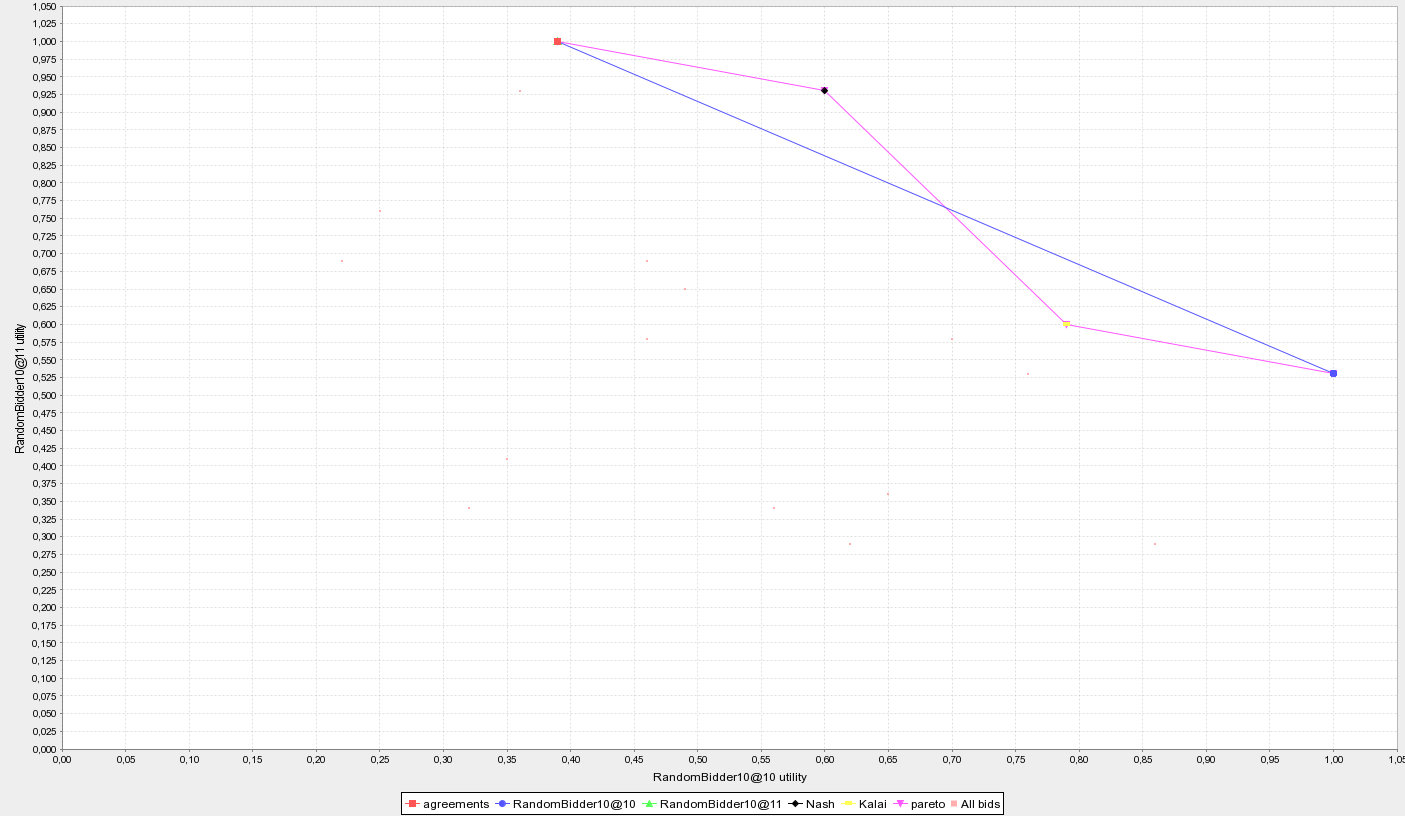
\includegraphics[width=0.45\linewidth]{report1/RB10vs10_100r.png}
  \caption{RandomBidderExample vs. RandomBidderExample with minimum target = 1. Both agents only make bids with their optimal utilities, until one of them accepts the other's bid. The pink line shows the pareto optimal frontier. }
  \label{fig:trials}
\end{figure}

\textbf{What would you argue is the most fair holiday arrangement for A and B?}\\
 There are multiple notions of fairness in game theory. Pareto efficiency, having the idea of social welfare as its foundation, can be seen as a form of fairness in the case of perfectly rational and self-interested agents. Humans, however, are not always rational and self-interested. Hence, if someone wants to model human decision making within a multi-agent system, he/she has to take fairness into account.\cite{Jong_Tuyls_Verbeeck_Roos}
According to de Jong, there two main motivations behind human fairness. First, \textbf{inequity aversion}, which explains people's revolt against inequitable outcomes. Second, \textbf{reciprocity}, which provides the possibility of rewarding and punishing one another. %De Jong uses these notions to describe the concept of priority awareness.
Another possibility that arises from the same motivations combines two ideas: \textbf{altruistic punishment} and \textbf{reputation}. The former refers to the appliance of punishment, even if the punisher does not benefit from it. The latter is constructed from previous interactions.\cite{Jong_Tuyls_Verbeeck_2008}
In our example, priority or reputation of the two agents is not known. Therefore, we will consider the \textbf{fairness equilibrium}, which was proposed by Rabin.\cite{Rabin_1993} This notion highlights the principle that when material payoffs are small enough, people sacrifice their own well being to reward or punish other people. With the assumption of equal weights per issue, we argue, the fairest outcome would be Antalya (as both would sacrifice something), 2 Weeks (as both agree on it) and 3-Star (as both sacrifice again). With unequal weights, as is the case here, another arrangement would also be sufficient. In the case of the described holiday scenario and given preferences, there is a clear higher weight in importance weighting for the type of hotel for agent A. A fair configuration would then include the location preference of agent A, resulting in a trip to Antalya for two weeks, in a hostel instead of a 3-star hotel. If there would be more issues, it would be fair if in return for this concession of agent B, the preference of agent B for another issue is chosen over the preference of agent A to make the complete arrangement more balanced.


\subsection{Interpretation of Results}

\textbf{Analyze the performance of the example agent \emph{RandomBidderExample}  against itself. Explain the outcome and how the agreement depends on the negotiation setting.}\\
Given the negotiation setting of \textbf{60 rounds} with two \textbf{RandomBidders} with \textbf{minimum target 0.8}, the pareto optimal outcome is not reached, as the agents do not reach an agreement. This is because the RandomBidderExample acceptance strategy always accepts the last bid, as long as at least 99 turns have been taken. Increasing the number of rounds to 100 resulted in a bid that was accepted with utilities 0.36096 and 0.93193. This was not pareto optimal. The bidding strategy of RandomBidderExample always generates bids that have a utility of at least the minimum target (0.8 here) for itself. 
%Thus, by chance the result could be pareto optimal if there is a set of preferences for which the utility of one of the agents is above the minimum target, and the utility for the other agent is sufficient to still reach pareto optimality. 
Thus, reaching pareto optimality depends on chance. This is further discussed below. There are multiple factors deciding the outcome of this negotiation. First, the preferences of the agents govern the shape of the pareto frontier. Second, the individual party strategies decide concession, bidding and acceptance behavior.
\newline %, evidenced by a change in preferences displayed in FIGURE X. Second, the chosen strategy of the agent which yields certain behavioural characteristics. In the case of the RandomBidderExample, the agent will always accept a bid if the number of rounds is set to at least 99, and won't accept otherwise. After setting the number of rounds to 99\\


\textbf{Now change the value of the MINIMUM\_TARGET of \emph{RandomBidderExample}; can you find a value for which a Pareto optimal outcome is reached?}\\
The minimum target is the minimum utility of the random bid the agent places. Consequently, the minimum target will govern the space of possible configurations of bids. If the minimum target for both agents is set sufficiently high, all bids will lie on the pareto frontier. Meaning, all possible configurations of bids for both agents, that have a utility over the given the minimum target value, are on the pareto efficient line. Whether both agents accept the bids only depends on the number of rounds the session will play, as established beforehand. Decreasing the minimum target results in a higher variance in the bids each agent does. Thus, decreasing the minimum target will decrease the chance of the final agreement being on the pareto frontier.\newline


\textbf{Analysis for \emph{BoulwareNegotiationParty} playing against \emph{ConcederNegotiationParty}.}\\
A Pareto Optimal Outcome is always reached, because the Conceder concedes with each subsequent round while the Boulware places the same bid with utility 1 every round. Hence, the Conceder will accept Boulware's bid if further concessions of its own bid's utility falls below the utility of the Boulware agent's bid. If the number of rounds played exceeds 1, the outcome of the negotiation does not change. In our session, this resulted in a utility of 1 for the Boulware, and a utility of 0.53260 for the Conceder. If only 1 round is played, the negotiation fails. We decided to investigate the Boulware's strategy further by analysing Boulware vs. Boulware. It seems as the Boulware strategies concession strategy depends on the number of rounds without changing bids (stagnation) and the remaining time. Hence, the Boulware never concedes against Conceder because the latter concedes every round and the negotiation does not stagnate. 

% INSERT ANSWER HERE\\
% Typically agree before max number of rounds reached, but number of rounds needed typically below the max. Shows some part of policy dependent on the number of rounds. Also, boulware never concedes, Conceder always just keeps making concessions until it reaches the maximum utility for boulware (bidding utility that boulware was bidding). This solution is thus far more preferable for boulware, but is pareto optimal for both Conceder and boulware.

% In boulware vs boulware, concessions are seemingly made only after a certain number of bids from the other opponent without changes. May be part of its base strategy.

% Generally, boulware's concession strategy seems to be dependent on the opponent's concession behavior.

% Likely keeps last concession value and tracks how long it has been since this has been lowered. If the opponent doesn't lower from this value after some amount of time, boulware will start conceding. \\
\renewcommand\refname{\scriptsize References\vspace*{-4mm}}
\bibliographystyle{plain}
{\footnotesize\bibliography{references}}



\end{document}
